\subsection{Convex subsets of a prehilbertian space}

If we calculate \(\|x - y\|^{2} = \langle x - y|x - y \rangle\) and \(\|x + y\|^{2} = \langle x + y|x + y \rangle\) for any two points x, y of a prehilbertian space E, we immediately get the « identity of the median »

\[
\left\| \frac {1}{2} (x + y) \right\| ^ {2} + \left\| \frac {1}{2} (x - y) \right\| ^ {2} = \frac {1}{2} (\| x \| ^ {2} + \| y \| ^ {2}).\tag{14}
\]

From this identity we deduce the following proposition :

\pandocbounded{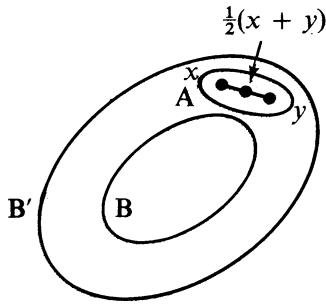
\includegraphics[keepaspectratio]{images/part002_56de9e6b.jpg}}\\
FIG. 1.

PROPOSITION 5. --- Let E be a prehilbertian space. Let d be a real number \textgreater0, δ a real number such that \(0 \leqslant \delta \leqslant d\) . Let B and B' be subsets of E defined by \(\|x\| < d\) , \(\| x\| \leqslant d + \delta\) respectively, and let A be a convex set contained in \(\mathbf{B}' - \mathbf{B}\) . Then for every pair of points \(x, y\) of A, we have \(\| x - y\| \leqslant \sqrt{12d\delta}\) (fig.~1).

In fact, we have \(\frac{1}{2} (x + y)\in \mathbf{A}\) , hence \(\| \frac{1}{2} (x + y)\| \geqslant d\) ; hence from (14) we get the inequality

\[
\left\| \frac {1}{2} (x - y) \right\| ^ {2} = \frac {1}{2} \left(\| x \| ^ {2} + \| y \| ^ {2}\right) - \left\| \frac {1}{2} (x + y) \right\| ^ {2} \leqslant (d + \delta) ^ {2} - d ^ {2} \leqslant 3 d \delta
\]

from which the proposition follows.

THEOREM 1. --- Let E be a prehilbertian space, and H a non-empty convex subset of E such that H is a Hausdorff and complete uniform subspace of E. For every \(x \in E\) , there exists a unique point \(p_{\mathrm{H}}(x)\) in H such that \(\|x - p_{\mathrm{H}}(x)\| = \inf_{y \in \mathrm{H}} \|x - y\|\) . The element \(p_{\mathrm{H}}(x)\) of H is also the unique element a of H satisfying the relation \(^{1}\)

\[
\mathcal {R} \langle x - a | y - a \rangle \leqslant 0\tag{15}
\]

for all \(y \in \mathbf{H}\) .

\pandocbounded{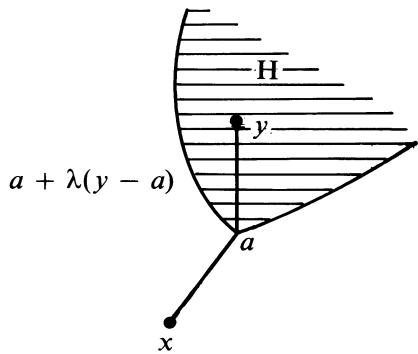
\includegraphics[keepaspectratio]{images/part002_6909685c.jpg}}\\
FIG. 2.

Put \(d = \inf_{y \in \mathbf{H}} \| x - y \|\) , and for every integer \(n > 0\) , let \(\mathrm{H}_n\) be the set of points \(y\) of \(\mathbf{H}\) such that \(\| x - y \| \leqslant d + n^{-1}\) . The set \(\mathrm{H}_n\) is closed in \(\mathbf{H}\) , is convex and non-empty, and its diameter is bounded by \(\sqrt{12d / n}\) for all large enough \(n\) , by prop. 5. The sequence \((\mathrm{H}_n)_{n \geqslant 1}\) being decreasing, and the set \(\mathbf{H}\) being Hausdorff and complete it follows that the base of the Cauchy filter \((\mathrm{H}_n)_{n \geqslant 1}\) converges to a point \(p_{\mathbf{H}}(x)\) of \(\mathbf{H}\) ; we have \(\{p_{\mathbf{H}}(x)\} = \bigcap_{n \geqslant 1} \mathrm{H}_n\) , hence \(p_{\mathbf{H}}(x)\) is the unique point \(a\) of \(\mathbf{H}\) such that \(\| x - a \| = d\) .

\(^{1}\) We recall (GT, VIII, § 1, No.~1) that \(\mathcal{R}(z)\) denotes the real part of the complex number z; we have \(\mathcal{R}(z)=z\) if z is real.

Let \(y \in H\) ; since \(H\) is convex, the point \(z(\lambda) = p_{\mathbf{H}}(x) + \lambda(y - p_{\mathbf{H}}(x))\) of \(E\) belongs to \(H\) for every real number \(\lambda\) such that \(0 < \lambda < 1\) . Hence we have

\[
\left\| x - z (\lambda) \right\| ^ {2} \geqslant \left\| x - p _ {\mathrm{H}} (x) \right\| ^ {2} \quad \text { for } \quad 0 <   \lambda <   1,
\]

which gives

\[
\mathcal {R} \left\langle x - p _ {\mathrm{H}} (x) \mid y - p _ {\mathrm{H}} (x) \right\rangle = \lim _ {\lambda \rightarrow 0} \frac {1}{2 \lambda} \left\{\| x - p _ {\mathrm{H}} (x) \| ^ {2} - \| x - z (\lambda) \| ^ {2} \right\} \leqslant 0.
\]

Conversely, let \(a\) be a point of \(\mathbf{H}\) such that \(\mathcal{R}\langle x - a|y - a\rangle \leqslant 0\) for all \(y\in \mathbf{H}\) . For every \(y\in \mathbf{H}\) , we have

\[
\left\| x - y \right\| ^ {2} = \left\| x - a \right\| ^ {2} + \left\| y - a \right\| ^ {2} - 2 \mathcal {R} \langle x - a | y - a \rangle \geqslant \left\| x - a \right\| ^ {2},
\]

and so \(\| x - a\| = d\) and finally that \(a = p_{\mathrm{H}}(x)\) follows from the first part of the proof. Q.E.D.

In what follows the mapping \(p_{H}\) of E in H will be called the projection from E onto H. We remark that \(p_{\mathrm{H}}(x)=x\) for all \(x\in H\) .

The first part of th. 1 is valid under more general hypotheses on the space E (V, p.~67, exerc. 31).

The proof of th. 1 establishes, among others, the following property :

COROLLARY 1. --- Let I be a set directed by a filter \(\mathfrak{F}\) and let \((y_i)_{i\in I}\) be a family of points of H. Let \(x\in E\) . Suppose that we have

\[
\lim _ {i, \mathfrak {F}} \| x - y _ {i} \| = \inf _ {z \in \mathrm{H}} \| x - z \|.
\]

Then \(y_{i}\) tends to \(p_{\mathrm{H}}(x)\) with respect to the filter \(\mathfrak{F}\) .

COROLLARY 2. --- For every x, y in E, we have

\[
\left\| p _ {\mathrm{H}} (x) - p _ {\mathrm{H}} (y) \right\| \leqslant \left\| x - y \right\|.
\]

In particular, the mapping \(p_{H}\) from E into H is continuous.

Let \(x, y\) be two points of \(E\) . Put \(a = p_{\mathrm{H}}(x) - x\) , \(b = p_{\mathrm{H}}(y) - p_{\mathrm{H}}(x)\) , \(c = y - p_{\mathrm{H}}(y)\) . By formula (15) (V, p.~10) we have \(\mathcal{R}\langle a|b\rangle \geqslant 0\) and \(\mathcal{R}\langle c|b\rangle \geqslant 0\) . We also have \(a + b + c = y - x\) , which gives,

\[
\| x - y \| ^ {2} = \| a + b + c \| ^ {2} = \| b \| ^ {2} + \| a + c \| ^ {2} + 2 \mathscr {R} \langle a | b \rangle + 2 \mathscr {R} \langle c | b \rangle
\]

\[
\geqslant \| b \| ^ {2} = \left\| p _ {\mathrm{H}} (x) - p _ {\mathrm{H}} (y) \right\| ^ {2}.
\]

This proves corollary 2.

PROPOSITION 6. --- Let E be a prehilbertian space and let \(\Phi\) be a non-empty, directed decreasing set of non-empty Hausdorff and complete convex subsets of E. For every \(x \in \mathrm{E}\) and every subset H of E, put \(d(x, \mathrm{H}) = \inf_{z \in \mathrm{H}} \| x - z \|\) . In order that the intersection M of the sets H belonging to \(\Phi\) be non-empty, it is necessary and sufficient that there exists \(x_0\) in E such that \(\sup_{\mathbf{H} \in \Phi} d(x_0, \mathbf{H})\) is finite. For every \(x \in \mathbf{E}\) we then have

\(p_{\mathbf{M}}(x) = \lim_{\mathrm{H}\in \Phi}p_{\mathrm{H}}(x)\) (limit with respect to the directed set \(\Phi\) ).

If \(\mathbf{M}\) is non-empty, \(d(x,\mathrm{H})\leqslant d(x,\mathbf{M})\) for all \(\mathbf{H}\in \Phi\) and all \(x\in \mathbb{E}\) .

Conversely, suppose that there exists a point \(x_0\) in \(\mathbf{E}\) and a real number \(\mathbf{C} \geqslant 0\) such that \(d(x_0, \mathbf{H}) \leqslant \mathbf{C}\) for all \(\mathbf{H} \in \Phi\) . Let \(x \in \mathbf{E}\) ; then

\[
d (x, \mathrm{H}) \leqslant \| x - x _ {0} \| + \mathrm{C} \quad \text { for   all } \quad \mathrm{H} \in \Phi ,
\]

hence the number \(d = \sup_{\mathbf{H} \in \Phi} d(x, \mathbf{H})\) is finite. Let \(\mathbf{B}\) be the set of all \(z \in E\) such that \(\| x - z\| \leqslant d\) . Since \(\mathbf{B}\) is convex and closed in \(\mathbf{E}\) , the sets \(\mathrm{H} \cap \mathrm{B}\) , for \(\mathrm{H}\) ranging over \(\Phi\) , are convex, Hausdorff and complete. Let \(\varepsilon > 0\) ; there exists a set \(\mathrm{H} \in \Phi\) such that \(d(x, \mathrm{H}) \geqslant \mathrm{d} - \varepsilon\) , and if \(\varepsilon < d/2\) , the diameter of \(\mathrm{H} \cap \mathrm{B}\) is bounded by \(\sqrt{12\varepsilon(d - \varepsilon)}\) by prop. 5 (V, p.~9). In other words, for all \(\mathrm{H}_0 \in \Phi\) , the closed sets \(\mathrm{H} \cap \mathrm{B}\) , for \(\mathrm{H} \in \Phi\) and \(\mathrm{H} \subset \mathrm{H}_0\) , form a base of the Cauchy filter on the Hausdorff and complete space \(\mathrm{H}_0\) . Hence the intersection of the sets \(\mathrm{H} \cap \mathrm{B}\) (for \(\mathrm{H} \in \Phi\) ) reduces to a point \(y\) . We get \(y \in \mathbf{M}\) and \(\| x - y \| = d = d(x, \mathbf{M})\) . Since \(\mathbf{M}\) is closed in \(\mathrm{H}_0\) , it is a Hausdorff, convex and complete set in \(\mathbf{E}\) , and so \(y = p_{\mathbf{M}}(x)\) . For every \(\mathrm{H} \in \Phi\) , we have \(p_{\mathrm{H}}(x) \in \mathrm{H} \cap \mathrm{B}\) , from which we get that \(p_{\mathbf{M}}(x) = \lim_{\mathrm{H} \in \Phi} p_{\mathrm{H}}(x)\) .

PROPOSITION 7. --- Let E be a Hausdorff prehilbertian space and let \(\Psi\) be a non-empty directed increasing set of non-empty, convex, complete subsets of E. Put \(A = \bigcup_{H \in \Psi} H\)

and suppose that the closure \(\mathbf{N}\) of \(\mathbf{A}\) is complete. Then \(\mathbf{N}\) is convex and we have \(p_{\mathrm{N}}(x) = \lim_{\mathrm{H}\in \Psi}p_{\mathrm{H}}(x)\) for all \(x\in \mathrm{E}\) .

It is clear that A is convex, hence its closure N is convex (II, p.~13). With the notations of prop. 6, \(d(x, \mathrm{N}) = \inf_{\mathrm{H} \in \Psi} d(x, \mathrm{H})\) , and consequently \(d(x, \mathrm{N})\) is the limit of \(d(x, \mathrm{H})\) with respect to the section filter of \(\Psi\) . Since \(p_{\mathrm{H}}(x) \in \mathrm{H}\) and

\[
\lim _ {\mathrm{H} \in \Psi} \| x - p _ {\mathrm{H}} (x) \| = \lim _ {\mathrm{H} \in \Psi} d (x, \mathrm{H}) = d (x, \mathrm{N}),
\]

it follows from cor. 1 of V, p.~11 that \(p_{\mathrm{H}}(x)\) tends to the projection \(p_{\mathrm{N}}(x)\) of \(x\) onto \(\mathbf{N}\) with respect to the section filter of \(\Psi\) .

